
\index{Sch\"{o}mann, Klaus}

\paragraph{Research Team}
Klaus Sch\"{o}mann (Professor), Anette Fasang (Doctoral Fellow), Sara-Izabella Geerdes (Doctoral Fellow), Liuben Siarov (Research Associate), Christoph Hilbert (Doctoral Fellow, Wissenschaftszentrum Berlin f\"{u}r Sozialforschung).

 Research in this area analyzes the links between lifelong learning and the labor market. We analyze sources of market failure, such as multiple factors responsible for underinvestment in lifelong learning. Persistent imbalances in supply and demand for training lead to a lack of participation in further training. In human capital theory, workers will invest until the marginal increase in wages equals the marginal cost of training. However, frequently there is no direct link between further training and returns to training (i.e., increase in wages or productivity) and workers therefore hesitate to take time out from the labor market to invest in training. The overdue change in reversing an ``early retirement culture'' in many European countries makes investment at later stages of the life course more attractive to employers and employees due to longer periods of returns on investments.

 Risk aversion and budgetary constraints in form of access to loans for purposes of learning also explain why people are reluctant to participate in training. Additionally firms might fear ``poaching'' of training costs of employees by other firms, although this problem can be addressed by adequate contractual arrangements.

 Further ways of tackling the barriers to participation in training are ensuring access to loans, promoting information availability, promoting transparency in training, certification and recognition of professional experience, targeting the groups least likely to participate by lifelong learning policies, the low-qualified and older workers. Research in these fields makes use secondary data analysis like panel data, large European surveys or own data collection through lab 3 resources like computer assisted telephone interviews. 

\textbf{Research Highlights 2006}

 Recent findings show that there are effective policies to reduce stigmatization of older workers and to combat the notion that older workers are less able or less willing to learn. Hence it is not only important to increase the budgets involved, but rather tackle the stigma that older people are less interested in learning. This complements the findings from the other disciplines, mainly psychology, in this area (see above).

 Drawing on the argument that lifelong learning provides mutual benefits to individuals, firms and society as a whole, innovative ways to co-finance lifelong learning are particularly promising policy solutions.

 Recently, we have started to investigate the ``function of learning in geographic and job mobility'' using the Eurobarometer 2005. This project is co-financed by the European Foundation for the improvement of living and working conditions based in Dublin. Our analyses show that skill development is an important element in the process of job mobility. Persons with higher investment in further training seem to be more mobile in the labor market and geographical mobility even across borders is highly linked to further training. The major driving force for participation in training over the last 12 months in the European Union, however, is a person's training initiated upon the employers' request (see Figure \ref{fig1:profKlausSchoemann}). A more proactive and self-motivated approach of individuals is needed to achieve high employment  rates also for older workers throughout the European Union. 

 The same European data source allows us to study various dimensions of job satisfaction across member states of the EU. So far we were able to demonstrate that satisfaction with training opportunities is an important element of overall satisfaction with a job and is part of the overarching domain of career prospects and work content as qualitative elements of a job.

\begin{figure}[ht]
  \begin{center}
    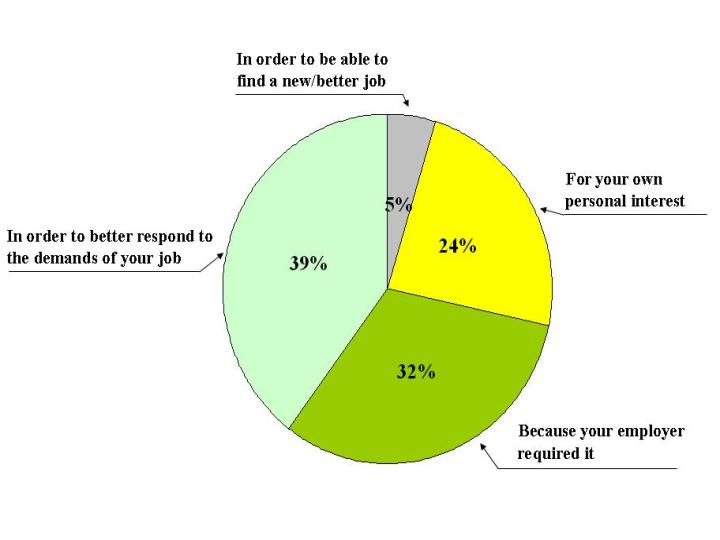
\includegraphics[width=7.5cm]{profKlausSchoemann-fig1.jpg}
    \caption{Reasons for taking part in training, EU 25 (Source: data from the Eurobarometer 2005, own calculations, Geerdes and Sch\"{o}mann 2006).}\label{fig1:profKlausSchoemann}
   \end{center}
\end{figure}

\newpage
\paragraph{Collaborations}
\begin{itemize}
\item Institute for Labour Studies (HIVA) \\ Catholic University Leuven \\ Dr. Tom Vandenberghe (co-ordinator)
\item Institute for Labour Studies (OSA) \\ University of Tilburg \\ Prof. Ruud Muffels 
\item Centre for Labour Market Policy Research (CAFO) \\ V\"axj\"o University \\ Prof. Dominique Anx\"o
\item Economic and Social Research Institute (ESRI), Dublin \\ Prof. Philip O'Connell 
\item Social Economic Research Rotterdam (SEOR) \\ University of Rotterdam \\ Prof. Jaap de Koning
\item Istituto per la Ricerca Sociale (IRS) Roma \\ Dr. Manuela Samek Hugo
\item Hugo Sinzheimer Institute (HSI) \\ University of Amsterdam \\ Prof. Ton Wilthagen; Dr. Els Sol
\item Institut f\"ur H\"ohere Studien (IHS), Wien \\ Prof Dr. Lorenz Lassnigg 
\item MATISSE, Centre National de la Recherche Scientifique, Paris I \\ Prof. Bernard Gazier
\item Institute for Employment Studies (IES) \\ University of Warwick \\ Prof. Ralf Rogowski 
\item McGill University, Canada \\ Prof. Axel van den Berg 
\item Universidad de Alcala, Madrid \\ Prof. Luis Toharia
\item Wissenschaftszentrum Berlin f\"ur Sozialforschung (WZB) \\ Prof. G\"unther Schmid 
\item Centre for Labour Market Research (CARMA) \\ Aalborg University \\ Prof. Per Madsen
\end{itemize}

\begin{bibunit}[apalike]
\nocite{*}
\putbib[profKlausSchoemann]
\end{bibunit}

\paragraph{Grants}

\begin{itemize}
\item European Foundation, 5th Framework Programme of the EU on ``managing social risks through transitional labour markets''. Co-financing by European Commission DG Employment as part of the mutual learning network. The research network consisted of 22 research groups in the European Union and a Canadian partner. The European Foundation in Dublin co-financed the data analysis of the Eurobarometer November 2005 data on labour mobility and geographical mobility in the EU. 
\item BMBF (PI: K. Sch\"omann): Qualification Needs in the OECD - Analysis and Implementation.
\end{itemize}